\section{Systematic Uncertainties}%
\label{sec:uncertainties}

The systematic uncertainties affecting the search for non-resonant and resonant
Higgs boson pair production are discussed in the following. Experimental
uncertainties are described in \Cref{sec:experimental_uncertainties} but exclude
uncertainties related to the estimation of \faketauhadvisC backgrounds in the
\hadhad channel. These were previously described
in~\Cref{sec:bkg_hadhad_ttbarfakes,sec:bkg_hadhad_ff}. Theory uncertainties are
described in~\Cref{sec:theory_uncertainties} and include uncertainties on the
modelling of physics processes using MC simulations.

The searches for Higgs boson pair production presented in this thesis are
generally limited by statistical uncertainties due to the finite number of
events observed in the SRs. Theory uncertainties play a lesser role and
instrumental uncertainties are only relevant for searches for scalar resonance
with low masses ($\mX \lesssim \SI{300}{\GeV}$). The impact of statistical and
systematic uncertainties on the results are discussed in the context of the
statistical interpretation in \Cref{sec:statistical_analysis}.


\subsection{Experimental Uncertainties}%
\label{sec:experimental_uncertainties}

Experimental uncertainties arise from the measurement of the integrated
luminosity, the re-weighting of the pile-up conditions in simulation, the
reconstruction of physics objects, and the efficiencies of selections applied to
these objects. Unless otherwise noted, all experimental uncertainties apply to
signal and background processes estimated using simulation.

% The integrated luminosity of the \pp~collision dataset recorded with the ATLAS
% detector during Run~2 of the LHC is measured with an uncertainty of
% \SI{1.7}{\percent}~\cite{ATLAS-CONF-2019-021}. This uncertainty is applied to
% all processes normalised using theoretical cross section predictions.
The uncertainty on the integrated luminosity of
\SI{1.7}{\percent}~\cite{ATLAS-CONF-2019-021} is applied to all processes
normalised using theoretical cross section predictions. Moreover, an uncertainty
is assigned on the re-weighting of the simulated event samples to match the
pile-up conditions in the recorded \pp~collision dataset. Uncertainties related
to the reconstruction and selection of physics objects are provided by dedicated
calibration measurements performed by the ATLAS collaboration. In this search,
these calibrations are used for electrons~\cite{EGAM-2018-01,TRIG-2018-05},
muons~\cite{MUON-2018-03}, \tauhadvis~\cite{ATLAS-CONF-2017-029},
jets~\cite{JETM-2018-05},
flavour-tagging~\cite{FTAG-2018-01,FTAG-2020-08,FTAG-2021-002}, and the
\pTmissAbs reconstruction~\cite{ATLAS-CONF-2018-023}. The calibration
measurements yield uncertainties on the momentum scale, momentum resolution, and
selection efficiency of reconstructed objects. The major categories of
instrumental uncertainties are summarised in
\Cref{tab:experimental_uncertainties_2}. Uncertainties on the selection
efficiencies of electron, muon, and \tauhadvis triggers are only considered in
channels where these triggers are used. All uncertainties affecting the
four-momentum of reconstructed and selected objects are also propagated to the
object-based \pTmissAbs reconstruction.
% Additional calibrations and uncertainties are derived for event samples using
% fast simulation of the ATLAS detector.

% Except for the luminosity uncertainty, any of the previously mentioned
% uncertainties can affect the shape and/or normalisation of the distributions
% used in the statistical interpretation. Therefore, both the shape and
% normalisation effects of these uncertainties are propagated to the relevant
% distributions.

\begin{table}[htbp]
  \centering

  \caption[Summary of instrumental uncertainties.]{Summary of instrumental
    uncertainties. The number of independent NPs describing the uncertainty is
    given in the right-most column.}%
  \label{tab:experimental_uncertainties_2}

  { \renewcommand{\arraystretch}{1.5} \begin{tabular}{lp{10.5cm}S[table-format=2.0]}
  \toprule
  Category    & Affected quantities & {$N_{\text{NPs}}$} \\
  \midrule
  Electrons   & Momentum scale and resolution; Reconstruction, identification, isolation, and trigger efficiencies. & 7 \\
  Muons       & Momentum scale and resolution; Reconstruction, track-to-vertex-association, isolation, and trigger efficiencies. & 15 \\
  \tauhadvis  & Momentum scale; Reconstruction, identification, $e$-veto, and trigger efficiencies; $e \to \tauhadvis$ mistag rates for $e$-veto.  & 38 \\
  Jets        & Momentum scale and resolution; Jet vertex tagging efficiency. & 48 \\
  $b$-tagging & Tagging efficiencies for $b$-jets and mistag rates for $c$- and light-quark jets. & 13 \\
  \pTmissAbs  & Momentum scale and resolution. & 3 \\
  \bottomrule
\end{tabular}


%%% Local Variables:
%%% mode: latex
%%% TeX-master: "../phd_thesis"
%%% End:
 }
\end{table}

Experimental uncertainties on the \faketauhadvisC background estimates in the
\lephad channels account for the statistical uncertainties of the \FFqcd,
\FFttbar, and \rqcd estimates. Moreover, uncertainties on the subtraction of
\ttbar and non-\ttbar processes in the combined FF method are taken into
account. An additional uncertainty is assigned on \rqcd due to it being derived
using a simulation-based estimate of the \ttbarFakes contribution in the \antiid
region. In the \lephad SLT and LTT channel, the total uncertainty on the
normalisation of the \faketauhadvisC background are
$^{\hspace{0.25pt}+\hspace{0.25pt}18\,\%}_{-23\,\%}$ and
$^{\hspace{0.25pt}+\hspace{0.25pt}28\,\%}_{-30\,\%}$, respectively. The effect
of these uncertainties on the shape of the final discriminants are considered in
the background model.

% The leading contributions to these uncertainties are the \ttbar subtraction
% and variations of \rqcd in the SLT channel and the \ttbar and non-\ttbar
% subtraction, variations of \rqcd, and the statistical precision of \FFttbar in
% the LTT channel. The effect of these variations on the shape of final
% discriminants are considered in the background model.


\subsection{Theory Uncertainties}%
\label{sec:modelling_uncertainties}%
\label{sec:theory_uncertainties}

A number of theoretical uncertainties need to be considered for signal and
background processes estimated using simulation. For a given process, these
uncertainties are split into uncertainties on the cross section and
uncertainties on the acceptance due to analysis selections. Generally,
acceptance uncertainties for a given signal or background process are assumed to
be correlated across regions if the uncertainty originates from the same source.

The description of the theory uncertainties is structured as follows: First, the
uncertainties on the major \ZHF and \ttbar backgrounds are described. Second,
uncertainties on minor background processes are estimated. Lastly, uncertainties
on the modelling of the signal processes are presented.


\subsubsection{Acceptance Uncertainties on \ZHF and \ttbar Backgrounds}

The normalisation of the \ZHF and \ttbar backgrounds are measured in the
simultaneous fit to observed data in all regions. Constraints on the
normalisation of the \ZHF background can be obtained from data in the
\ZHF~CR. Similarly, the \ttbar normalisation can be constrained in the SR of the
\lephad SLT channel and the \ZHF~CR. Since the normalisation of these processes
is determined in the fit to data, any uncertainties on the normalisation
(e.g.~cross section uncertainties) are omitted. Instead, uncertainties on the
relative acceptance of \ZHF and \ttbar between analysis regions have to be
considered. These uncertainties are hereafter referred to as \emph{relative
  acceptance uncertainties}.
% The approach outlined below was originally adopted by the previous search
% performed in this channel~\cite{HIGG-2016-16-witherratum} from searches and
% measurements of $VH$~($H\to\bbbar$)
% production~\cite{HIGG-2016-29,HIGG-2018-04,HIGG-2018-51}.

The derivation of relative acceptance uncertainties is described using an
example of a background that is estimated using simulation and normalised by a
fit to data in two regions~A and~B, with region~A being declared as the
\emph{reference region}. The probability of an event being selected into
region~R is given by the product of acceptance and efficiency,
$(\AccTimesEff)_{\text{R}}$, for this region. The simulation of the background
process predicts how \AccTimesEff relates between regions and one can define the
ratio
\begin{align*}
  \mathcal{R} = \frac{(\AccTimesEff)_{\text{B}}}{(\AccTimesEff)_{\text{A}}} \,\text{,}
\end{align*}
which is referred to as the \emph{relative acceptance} between regions~A
and~B. Uncertainties on the modelling of $\mathcal{R}$ in simulation are
assigned as uncertainties on the normalisation of the background process in
region~B and no additional uncertainties are assigned in the reference
region. Uncertainties on $\mathcal{R}$ are estimated by performing variations of
the simulation and estimating a relative change in $\mathcal{R}$ according to
\begin{align}
  \frac{\Delta \mathcal{R}}{\mathcal{R}} = \frac{\mathcal{R}(\text{variation}) - \mathcal{R}(\text{nominal})}{\mathcal{R}(\text{nominal})} \,\text{,}
  \label{eq:relative_acceptance_uncertainty}
\end{align}
where $\mathcal{R}(\text{nominal})$ and $\mathcal{R}(\text{variation})$ is the
relative acceptance predicted by the nominal and varied simulation setup,
respectively. Using relative acceptances to define modelling uncertainties leads
to cancellations of variations that lead to the same relative change in
\AccTimesEff in both regions. This corresponds to an overall change in
normalisation of the process in both regions that can be absorbed into the free
normalisation factor.

% This uncertainty on the relative acceptance between the the
% reference region A and region B is included in the background model
% by assigning a normalisation uncertainty of
% $\Delta \mathcal{R} / \mathcal{R}$ on the background in region B.

% The absolute value\footnote{When introducing multiple regions, the
% relative sign of $\Delta \mathcal{R} / \mathcal{R}$ when comparing
% different regions to the same reference is important when
% correlating these uncertainties in the statistical analysis and is
% kept to allow to consistently define the variations.} of
% $\Delta \mathcal{R} / \mathcal{R}$ is considered the extrapolation
% uncertainty.

% The shape effects of uncertainties are estimated separately and will be described in~\Cref{sec:modelling_uncertainties}.

Relative acceptance uncertainties are defined for the \ZHF and \ttbar
backgrounds using the \ZHF~CR as a reference region. The uncertainties are
estimated separately for the SRs of the \hadhad, \lephad SLT, and \lephad LTT
channel.

For the \ZHF background, the uncertainties are derived by performing variations
of the simulation setup following recommendations by the ATLAS collaboration,
which are summarised in \Cref{app:zjets_uncertainties}. The following aspects of
the simulation are varied: the matrix element generator and parton shower
program, the factorisation and renormalisation scales, the resummation scale,
the multi-jet merging scale, the PDFs and \alphas, and the PDF set. The relative
acceptance uncertainties on the \ZHF background are summarised
in~\Cref{tab:uncertainties_zhf_extrapol} for the three SRs.

A similar approach is taken for the \ttbar background. Variations of the
simulation setup are performed according to prescriptions developed by the ATLAS
collaboration, which are documented in~\Cref{app:top_uncertainties}. The
following elements of the simulation setup are varied: the matrix element
generator, the simulation of the parton shower and hadronisation model, the
factorisation and renormalisation scales, the simulation of initial- and
final-state radiation, the PDFs and \alphas. The relative acceptance
uncertainties resulting from these prescriptions are summarised
in~\Cref{tab:uncertainties_ttbar_extrapol}.

\begin{table}[htbp]
  \centering

  \caption[Relative acceptance uncertainties on the \ZHF and \ttbar background
  in the SRs.]{Relative acceptance uncertainties on the \ZHF (a) and \ttbar (b)
    background in the three SRs. All uncertainties are estimated using the
    \ZHF~CR as the reference region. The relative sign of the effect of
    variations is indicated by the $\pm$ and $\mp$ prefixes. The total
    uncertainty is given for illustration purposes only.}

  \begin{subtable}[t]{0.95\textwidth}
    \centering
    \subcaption{\ZHF background}%
    \label{tab:uncertainties_zhf_extrapol}

    \begin{tabular}{lccc}
  \toprule
  & \multicolumn{3}{c}{Signal region} \\
  \cline{2-4}
  Uncertainty source & {\hadhad} & {\lephad SLT} & {\lephad LTT} \\
  \midrule
  \MGNLO+\PYTHIA[8] & $\pm 7.0\,\%$ & $\mp 2.1\,\%$ & $\mp 11\,\%$ \\[0.2em]
  Factorisation and renormalisation scale & $\substack{+12 \\ -9.7}\,\%$ & $\substack{+5.4 \\ -3.0}\,\%$ & $\substack{+8.5 \\ -3.0}\,\%$ \\[0.2em]
  Multi-jet merging (CKKW) & $\pm 5.4\,\%$ & $\pm 7.0\,\%$ & $\pm 7.2\,\%$ \\[0.2em]
  Parton shower resummation scale (QSF) & $\mp 6.0\,\%$ & $\pm 1.7\,\%$ & $\pm 1.6\,\%$ \\[0.2em]
  Alternative PDF sets & $\pm 1.0\,\%$ & $ \pm 1.0\,\%$ & $\pm 1.1\,\%$ \\[0.2em]
  PDF+\alphas (\NNPDF[3.0nnlo]) & $\pm 0.77\,\%$ & $\pm 0.27\,\%$ & $\pm 0.35\,\%$ \\
  \midrule
  Total & $\substack{+16\\-15}\,\%$ & $\substack{+9.3\\-8.1}\,\%$ & $\substack{+16\\-14}\,\%$ \\
  \bottomrule
\end{tabular}

%%% Local Variables:
%%% mode: latex
%%% TeX-master: "../phd_thesis"
%%% End:

  \end{subtable}

  \vspace{12pt}

  \begin{subtable}[t]{0.95\textwidth}
    \centering
    \subcaption{\ttbar background}%
    \label{tab:uncertainties_ttbar_extrapol}

    \begin{tabular}{lccc}
  \toprule
  & \multicolumn{3}{c}{Signal region} \\
  \cline{2-4}
  Uncertainty source & {\hadhad} & {\lephad SLT} & {\lephad LTT} \\
  \midrule
  ME & $\mp 3.8\,\%$ & $\mp 0.3\,\%$ & $\pm 0.9\,\%$ \\[0.2em]
  PS & $\pm 2.2\,\%$ & $\pm 7.2\,\%$ & $\pm 8.8\,\%$ \\[0.2em]
  ISR & $\mp 0.3\,\%$ & $\mp 0.9\,\%$ & $\pm 1.3\,\%$ \\[0.2em]
  FSR & $\substack{-4.5\\+2.0}\,\%$ & $\substack{-1.0\\+1.5}\,\%$ & $\substack{-3.2\\+1.0}\,\%$ \\[0.2em]
  PDF+\alphas & $\pm 0.2\,\%$ & $\pm 0.6\,\%$ & $\pm 0.8\,\%$ \\
  \midrule
  Total & $\substack{+4.8\\-6.3}\,\%$ & $\pm 7.4\,\%$ & $\substack{+9.0\\-9.4}\,\%$ \\
  \bottomrule
\end{tabular}

%%% Local Variables:
%%% mode: latex
%%% TeX-master: "../phd_thesis"
%%% End:

  \end{subtable}
\end{table}

Relative acceptance uncertainties are implemented as uncertainties on the
normalisation of backgrounds in the SRs. Variations of the modelling in
simulation can also change the shapes of discriminants used for signal
extraction, including $\mll$ in the \ZHF CR, which need to be
considered. Therefore, the impact of modelling uncertainties on the
distributions of the MVA discriminants in the SRs and the \mll distribution in
the \ZHF~CR are investigated. In cases where the shapes do not differ
significantly, no additional uncertainties are assigned. When deviations are
observed, the shape uncertainties are propagated to the discriminants and
correlated with the corresponding normalisation uncertainties.

Shape uncertainties on the \ZHF background are considered for the variation of
the matrix element generator and parton shower program (\hadhad channel), and
for variations of the factorisation and renormalisation scales (\hadhad and
\lephad SLT/LTT channels). All other variations are found to have negligible
impact on the shape of the discriminating variables, including \mll in the
\ZHF~CR.

Shape uncertainties on the \ttbar background are considered for the comparison
with an alternative matrix element generator and parton shower program (\hadhad
and \lephad SLT channels), and the uncertainty on the modelling of initial- and
final-state radiation (\hadhad channel). All other variations have negligible
impact on the shapes of the relevant distributions.


\subsubsection{Uncertainties on Minor Backgrounds}

The minor backgrounds considered in the analysis are normalised using
theoretical cross sections predictions and thus both cross section and
acceptance uncertainties are considered. Except for the $tW$~acceptance
uncertainties, only uncertainties on the normalisation of minor backgrounds are
considered. A brief description of the uncertainties on minor backgrounds is
given in the following:
\begin{description}

\item[\PZ + LF] A normalisation uncertainty of \SI{5}{\percent} is assigned to
  account for the uncertainty on the predicted cross section of \Zjets
  production at NNLO~\cite{Anastasiou:2003ds}. Additionally, an acceptance
  uncertainty of \SI{23}{\percent} is adopted from Ref.~\cite{HIGG-2018-51}.

\item[\PW + jets] A \SI{5}{\percent} cross section uncertainty is assigned to
  the NNLO cross section prediction~\cite{Anastasiou:2003ds}. A normalisation
  uncertainty of \SI{37}{\percent} is assigned in the \lephad channels, which is
  adopted from Ref.~\cite{HIGG-2018-51}. This uncertainty is inflated to
  \SI{50}{\percent} in the \hadhad channel since the small \Wjets contribution
  is not part of the data-driven \faketauhadvisC estimation.

\item[Diboson] Normalisation uncertainties of \SI{20}{\percent},
  \SI{26}{\percent}, and \SI{25}{\percent} are applied to $ZZ$, $WZ$, and $WW$
  production, respectively. These uncertainties are adopted from
  Ref.~\cite{HIGG-2018-51}.

\item[Single top quark] Uncertainties on the cross section used to normalise the
  predictions are taken from Ref.~\cite{stopxsec}. An acceptance uncertainty of
  \SI{20}{\percent} is assigned to the minor contribution of single-top-quark
  production via $s$- and $t$-channel diagrams, which is adopted from
  Ref.~\cite{HIGG-2018-51}.

  Acceptance uncertainties in the phase space selected by the analysis are
  derived for $tW$~production, which is the dominant source of single-top-quark
  background in this analysis. The acceptance uncertainties from the NLO+PS
  matching and the choice of parton shower program are estimated by comparison
  with alternative simulation setups using \MGNLO and \HERWIG[7],
  respectively. Uncertainties from PDF+\alphas and the simulation of initial-
  and final-state radiation are obtained by re-weighting of the nominal
  simulation result. Finally, an uncertainty on the treatment of the
  interference between $tW$ production at NLO and \ttbar production is estimated
  by performing MC-to-MC comparisons of the nominal \emph{diagram removal} and
  \emph{diagram subtraction} schemes~\cite{Frixione:2008yi}.

  The total acceptance uncertainty on $tW$~production is \SI{34}{\percent} in
  the \hadhad~channel, \SI{14}{\percent} in the \lephad~SLT channel, and
  \SI{23}{\percent} in the \lephad~LTT channel. Shape effects of the final-state
  radiation and $tW$-$\ttbar$ interference uncertainties on the MVA
  discriminants are taken into account in the background model.

\item[Single SM~$H$] Uncertainties on the total cross section of the SM $H$
  production modes considered as backgrounds are assigned according to the
  recommendations in Ref.~\cite{deFlorian:2016spz_book} for
  $m_{H} = \SI{125.0}{\GeV}$. Uncertainties on the branching ratios of
  $\PHiggs \to \tautau$ and $\PHiggs \to \bbbar$ are assigned to the relevant
  processes and are taken from Ref.~\cite{deFlorian:2016spz_book}.

  An acceptance uncertainty of \SI{100}{\percent} is assigned to $H \to \tautau$
  backgrounds produced via \ggF, VBF, and $WH$ to account for difficulties in
  the modelling of associated production of SM~$H$ with heavy-flavour
  quarks. This uncertainty is a convention adopted by the ATLAS collaboration
  for searches for Higgs boson pair production using the \pp~collision dataset
  collected during Run~2 of the LHC.

  Acceptance uncertainties in the phase space selected by the analysis are
  derived for single-Higgs-boson backgrounds produced via $ZH$ and $\ttbar H$
  for both $H \to \tautau$ and $H \to \bbbar$. They are derived by varying the
  parton shower program, the factorisation and renormalisation scale, the PDFs
  and \alphas. Additionally, uncertainties on the NLO+PS matching and the
  modelling of initial- and final-state radiation are assigned to the $\ttbar H$
  background.
\end{description}

% \begin{table}[htbp]
%   \centering

%   \missingfigure[figwidth=0.75\textwidth]{Summary of bkg uncertainties.}

%   \caption{Summary of minor background uncertainties}
% \end{table}


\subsubsection{Signal Modelling Uncertainties: SM~$HH$ Production}

Uncertainties on the predicted SM~\HH production cross section are taken into
account when the signal strength is used as the POI in the statistical
analysis. In contrast, when the SM~\HH production cross section is the POI,
cross section uncertainties on the signal processes are omitted. In either case,
uncertainties on the branching ratios of $H \to \tautau$ and $H \to \bbbar$ are
taken from Ref.~\cite{deFlorian:2016spz_book} and assigned as uncertainties on the
signal normalisation.

The uncertainty on the SM~\HH production cross section via \ggF
is~$^{\hspace{0.25pt}+\hspace{0.25pt}\phantom{2}6}_{-23}\valuesep\si{\percent}$
for the scale variations and the treatment of the finite top-quark
mass~\cite{Baglio:2020wgt}, and~\SI{\pm 3.0}{\percent} for variations of
PDF+\alphas~\cite{LHCHWGHH}. Similarly, the uncertainty on the SM~\HH production
cross section via VBF
is~$^{\hspace{0.25pt}+\hspace{0.25pt}0.03}_{-0.04}\valuesep\si{\percent}$ for
the scale variations and \SI{\pm 2.1}{\percent} for variations of
PDF+\alphas~\cite{LHCHWGHH}.

Signal acceptance uncertainties are derived in all SRs by performing variations
of the generator setup. An uncertainty on the choice of parton shower and
hadronisation model is estimated by comparing the nominal setup using \PYTHIA[8]
with an alternative setup using \HERWIG[7] for parton showering and
hadronisation. An uncertainty from missing higher orders of the truncated
perturbative expansion in \alphas is estimated by performing six variations of
the factorisation and renormalisation scales. For SM~\HH production via \ggF
(VBF), uncertainties on the PDFs are taken into account following the
prescriptions of the \PDFforLHC[15nlo]~\cite{Butterworth:2015oua}
(\NNPDF[3.0nlo]~\cite{Ball:2014uwa}) set of PDFs. Lastly, the value
of~$\alphas\mathopen{}\bigl( Q^2 = \mZ^2 \bigr)\mathclose{}$ is varied up and
down by $0.0015$ ($0.001$) about the central value of $0.118$ in the
\PDFforLHC[15nlo] (\NNPDF[3.0nlo]) PDF set. The SM~$HH$ acceptance uncertainties
are summarised in~\Cref{tab:theory_uncertainty_signal} for the \ggF and VBF
production modes.

% The uncertainties on PDF+\alphas are found to be negligible in most cases and
% thus omitted. The impact of the variations on the shape of the MVA
% discriminants is found to be negligible in most cases. The variations of the
% factorisation and renormalisation scales for the VBF production mode in the
% \hadhad SR is found to induce small changes in the shape (up to
% \SI{2}{\percent} in bins sensitive to the SM $HH$ signal) of the SM $HH$ BDT
% score distribution, which is implemented as a shape uncertainty for later
% statistical evaluation.

\begin{table}[htbp]
  \centering

  \caption[Unceratinties on the acceptance of SM~\HH events in the
  SRs.]{Uncertainties on the acceptance of SM~\HH events produced via \ggF and
    VBF in the three SRs. Uncertainties marked as ``--'' are found to be
    negligible.}%
  \label{tab:theory_uncertainty_signal}

  \begin{tabular}{l
  S[retain-explicit-plus]
  S[retain-explicit-plus]
  S[retain-explicit-plus]}
  \toprule
  & \multicolumn{3}{c}{Acceptance uncertainty / \%} \\
  \cmidrule{2-4}
  Source & {\hadhad} & {\lephad SLT} & {\lephad LTT} \\
  \midrule
  \multicolumn{4}{c}{SM $HH$ (ggF production mode)} \\
  \midrule
  Parton shower       & \pm 4.3 & \pm 7.6 & \pm 7.5 \\
  Scales (\muF, \muR) & \pm 1.4 & \pm 1.2 & \pm 1.0 \\
  PDF+\alphas & {--} & {--} & {--} \\
  \midrule
  \multicolumn{4}{c}{SM $HH$ (VBF production mode)} \\
  \midrule
  Parton shower & \pm 3.0 & \pm 6.3 & \pm 2.1 \\
  Scales (\muF, \muR) & {--$^\dagger$} & \pm 1.0 & \pm 1.0 \\
  PDF+\alphas & \pm 1.0 & {--} & {--} \\
  \bottomrule
\end{tabular}

%%% Local Variables:
%%% mode: latex
%%% TeX-master: "../phd_thesis"
%%% End:

\end{table}


\subsubsection{Signal Modelling Uncertainties: Resonant \HH Production}

Cross section uncertainties are not considered for signals from resonant \HH
production due to the cross section~$\sigma(pp \to X \to HH)$ being used as the
POI. However, uncertainties on the Higgs boson branching ratios are considered.

Signal acceptance uncertainties are estimated for the choice of parton shower
and hadronisation model, the factorisation and renormalisation scales, and
PDF+\alphas. These uncertainties are derived for a subset of resonance masses
considered in the analysis
% (due to the availability of alternative samples)
which are then extrapolated to the full set.

The acceptance uncertainty from the choice of parton shower program and
hadronisation model is estimated by comparing the default configuration using
\HERWIG[7] with \PYTHIA[8] for signals with
\mbox{$\mX / \si{\GeV} \in \left\{ 251, 260, 280, 400, 500, 1000 \right\}$}.
% \begin{align*}
%   \mX / \si{\GeV} \in \left\{ 251, 260, 280, 400, 500, 1000
%   \right\} \,\text{.}
% \end{align*}
% The uncertainty is estimated by comparing the acceptance of signal-like
% events, which for this purpose are defined as all events exceeding the
% 15\textsuperscript{th} percentile of the PNN score distribution for the
% default signal generation setup, between both parton shower programs. This
% approach is taken due to large changes in acceptance of (background-like)
% signal events at low PNN score to which this search is not sensitive, thus
% avoiding an inflation of the parton shower uncertainty at high PNN score which
% the analysis can be sensitive to.
The uncertainties evaluated at these points are linearly interpolated
(extrapolated) for $\mX \leq \SI{1000}{\GeV}$ ($\mX > \SI{1000}{\GeV}$) to
provide estimates of the uncertainty for other mass points. This procedure is
illustrated in \Cref{fig:resonant_partonshower} for all three channels. The
extrapolation to $\mX = \SI{1600}{\GeV}$ can lead to an uncertainty of up to
\SI{20}{\percent}.

% The alternative configuration using \PYTHIA for parton showering predicts
% acceptances that are slightly larger than the nominal configuration for the
% \hadhad and \lephad SLT channels at low resonance masses. For
% $\mX = \SI{1000}{\GeV}$ \HERWIG predicts larger signal acceptances in all
% three channels. The linear extrapolation in \mX to the largest resonance mass
% of \SI{1600}{\GeV} that is considered leads to acceptance uncertainties
% ranging from \SIrange[range-units=single]{16}{19}{\percent}.

\begin{figure}[htbp]
  \centering

  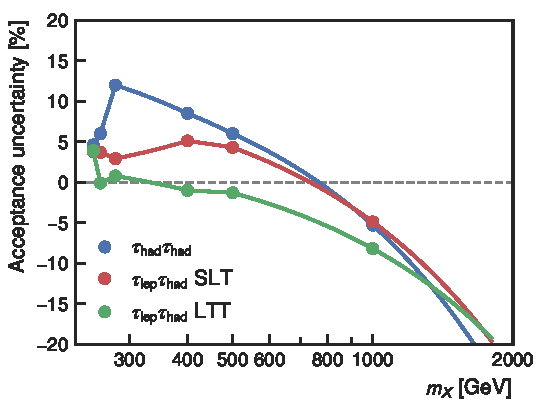
\includegraphics[scale=0.85]{uncertainties/resonant_ps_acc}

  \caption[Uncertainties on the acceptance of $pp \to X \to \HH$ events in the
  SRs due to the choice of parton shower and hadronisation model.]{Uncertainties
    on the acceptance of $pp \to X \to \HH$ events in the SRs due to the choice
    of parton shower and hadronisation model. A positive (negative) sign of the
    uncertainty indicates that the alternative configuration (\PYTHIA) predicts
    a larger (smaller) \AccTimesEff than the nominal one (\HERWIG). The lines
    indicate the linear inter-/extrapolation used to obtain the uncertainties
    for other mass points considered in the analysis.}%
  \label{fig:resonant_partonshower}
\end{figure}

Acceptance uncertainties from factorisation and renormalisation scales as well
as PDF+\alphas are evaluated at generator-level for two mass points with
$\mX = \SI{500}{\GeV}$ and \SI{1000}{\GeV} after approximating the selections
applied in the analysis. The uncertainties are found to be negligible and are
therefore omitted.

An additional uncertainty is assigned in the \hadhad and \lephad LTT channels to
signal samples using fast simulation of the ATLAS detector. The efficiency of
\tauhadvis-triggers is found to deviate between full and fast simulation,
without dedicated calibrations of \tauhadvis-trigger efficiencies in fast
simulation being available. An uncertainty is estimated by comparing the
acceptance between full and fast simulation for a benchmark signal with
$\mX = \SI{400}{\GeV}$. The acceptance predicted using fast simulation is
\SI{6.5}{\percent} (\SI{3.6}{\percent}) larger than in full simulation for the
\hadhad (\lephad LTT) SR for the benchmark point. Distributions of kinematic and
MVA input variables are compared between fast and full simulation showing no
significant deviations in their shapes. Therefore, the difference in acceptance
is assigned as an additional normalisation uncertainty in the \hadhad and
\lephad LTT channel for all signal samples using fast detector simulation, i.e.\
all signals with $\mX \leq \SI{1000}{\GeV}$.

%%% Local Variables:
%%% mode: latex
%%% TeX-master: "../../phd_thesis"
%%% End:
